\documentclass[aspectratio=169, 10pt]{beamer}

% ---------- Tema y colores ----------
\usetheme{default}
\usecolortheme{default}
\setbeamertemplate{navigation symbols}{}
\setbeamertemplate{footline}[frame number]
\setbeamertemplate{frametitle continuation}{}

\definecolor{StanfordRed}{RGB}{140,21,21}
\definecolor{StanfordGray}{RGB}{77,77,77}
\definecolor{LightGray}{RGB}{240,240,240}
\definecolor{AccentBlue}{RGB}{0,84,166}
\definecolor{AccentGreen}{RGB}{0,130,100}
\definecolor{UCMBlue}{RGB}{4, 171, 226}
\definecolor{UCMNavy}{RGB}{20, 65, 134}

\setbeamercolor{frametitle}{fg=white, bg=UCMBlue}
\setbeamercolor{title}{fg=white}
\setbeamercolor{author}{fg=white}
\setbeamercolor{institute}{fg=white!80}
\setbeamercolor{structure}{fg=UCMBlue}
\setbeamercolor{block title}{bg=UCMBlue!15!white, fg=UCMBlue}
\setbeamercolor{block body}{bg=LightGray}
\setbeamercolor{alerted text}{fg=UCMBlue}
\setbeamercolor{example text}{fg=UCMBlue}

\setbeamerfont{frametitle}{series=\bfseries, size=\large}
\setbeamerfont{title}{series=\bfseries, size=\LARGE}
\setbeamerfont{block title}{series=\bfseries}

% ---------- Paquetes ----------
\usepackage[utf8]{inputenc}
\usepackage[T1]{fontenc}
\usepackage[provide=*,spanish]{babel}
\usepackage{amsmath, amssymb, bm}
\usepackage{algorithmic}
\usepackage{tikz}
\usepackage{pgfplots}
\pgfplotsset{compat=1.18}
\usetikzlibrary{arrows.meta, shapes.geometric, positioning, fit, calc,
	decorations.pathreplacing, backgrounds, shadows, patterns}
\usepackage{booktabs}
\usepackage{xcolor}
\usepackage{multicol}
\usepackage{tcolorbox}
\tcbuselibrary{skins, breakable}

% ---------- Comandos útiles ----------
\newcommand{\R}{\mathbb{R}}
\newcommand{\E}{\mathbb{E}}
\newcommand{\Var}{\operatorname{Var}}
\newcommand{\relu}{\operatorname{ReLU}}
\newcommand{\sgn}{\operatorname{sign}}
\newcommand{\h}{\bm{h}}
\newcommand{\x}{\bm{x}}
\newcommand{\W}{\bm{W}}
\newcommand{\bb}{\bm{b}}
\newcommand{\X}{\bm{X}}
\newcommand{\Hb}{\bm{H}}
\newcommand{\Ob}{\bm{O}}

\newcommand{\formula}[1]{%
	\begin{tcolorbox}[colback=UCMBlue!8, colframe=UCMBlue, arc=4pt,
		boxsep=2pt, left=6pt, right=6pt, top=3pt, bottom=3pt]
		#1
	\end{tcolorbox}
}

% ---------- Portada ----------
\title{\textbf{Redes Neuronales}}
\subtitle{El Perceptr\'on Multicapa (MLP)}
\author{Sergio Hern\'andez\\ shernandez@ucm.cl}
\institute{
	% --- Para restaurar el logo institucional, reemplace este tikzpicture por:
	% \includegraphics[width=4cm, height=2cm]{figures/mindslab.png}
	\begin{tikzpicture}[scale=0.42, every node/.style={transform shape}]
		\foreach \i/\y in {1/0,2/1,3/2}{\node[circle,draw=white,fill=white!20,minimum size=4mm] (i\i) at (0,\y){};}
		\foreach \i/\y in {1/-0.5,2/0.5,3/1.5,4/2.5}{\node[circle,draw=white,fill=white!35,minimum size=4mm] (h\i) at (2,\y){};}
		\foreach \i/\y in {1/0.5,2/1.5}{\node[circle,draw=white,fill=white!50,minimum size=4mm] (o\i) at (4,\y){};}
		\foreach \a in {1,2,3}\foreach \b in {1,2,3,4}{\draw[white,opacity=0.5] (i\a)--(h\b);}
		\foreach \a in {1,2,3,4}\foreach \b in {1,2}{\draw[white,opacity=0.5] (h\a)--(o\b);}
	\end{tikzpicture}
	\\ \textbf{Universidad Cat\'olica del Maule}}
\date{}


\begin{document}
% --- Título ---
{
	\setbeamertemplate{background}{
		\begin{tikzpicture}[remember picture, overlay]
			\fill[UCMBlue] (current page.south west) rectangle (current page.north east);
			\fill[UCMBlue!70!black, opacity=0.5]
			(current page.south west) -- ++(0,3) -- ++(18,0) -- cycle;
			\foreach \i in {1,...,40}{
				\fill[white, opacity=0.04]
				({random()*17}, {random()*10}) circle ({random()*0.3});
			}
		\end{tikzpicture}
	}
	\begin{frame}[plain]
		\vspace{1.2cm}
		\titlepage
		\begin{tikzpicture}[remember picture, overlay]
			\node[white, opacity=0.15, font=\fontsize{80}{80}\selectfont]
			at (current page.east) [xshift=-2cm] {$\sigma$};
		\end{tikzpicture}
	\end{frame}
}


%=====================================================================
\section{Motivaci\'on: del modelo lineal a la red profunda}
%=====================================================================

\begin{frame}
\frametitle{Hacia la primera red \emph{profunda}}
\begin{itemize}
	\item Los modelos lineales (regresi\'on lineal, \emph{softmax}) suponen una relaci\'on \textbf{af\'in} entre las entradas y la salida.
	\pause
	\item Linealidad implica \textbf{monotonicidad}: aumentar una variable siempre mueve la predicci\'on en la misma direcci\'on. Esto es a menudo falso.
	\begin{itemize}
		\item \emph{Ejemplo}: la probabilidad de impago no crece de forma lineal con el ingreso; los p\'ixeles de una imagen no determinan la categor\'ia de forma af\'in.
	\end{itemize}
	\pause
	\item \textbf{Idea central}: apilar varias capas de neuronas, cada una \emph{totalmente conectada} a la anterior, e intercalar \emph{no linealidades}.
	\pause
\end{itemize}
\begin{block}{Perceptr\'on multicapa (MLP)}
La red profunda m\'as simple: capas de neuronas donde cada una recibe de la capa inferior e influye en la superior. Con suficientes neuronas y datos, aprende relaciones que un modelo lineal no puede representar.
\end{block}
\end{frame}

\begin{frame}
\frametitle{Arquitectura de un MLP con una capa oculta}
\begin{columns}[T]
\begin{column}{5.2cm}
\begin{itemize}
	\item \textbf{Capa de entrada}: no realiza c\'alculo, s\'olo distribuye $\x$.
	\item \textbf{Capa oculta}: neuronas con activaci\'on no lineal.
	\item \textbf{Capa de salida}: produce la predicci\'on $\Ob$.
	\item Es una red \emph{totalmente conectada} (\emph{fully connected}): cada neurona se une a todas las de la capa vecina.
\end{itemize}
\end{column}
\begin{column}{6.5cm}
\begin{center}
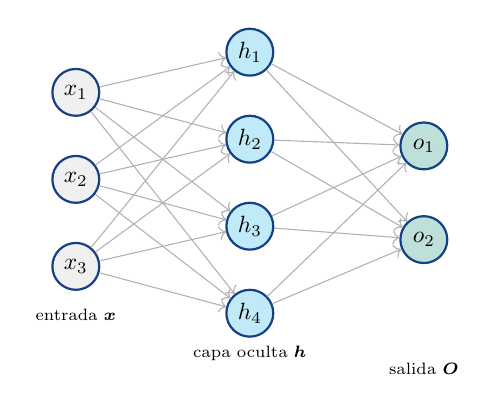
\begin{tikzpicture}[scale=0.85, transform shape,
	neuron/.style={circle,draw=UCMNavy,thick,minimum size=7mm,inner sep=0pt},
	inp/.style={neuron,fill=LightGray},
	hid/.style={neuron,fill=UCMBlue!25},
	outl/.style={neuron,fill=AccentGreen!25}]
% input layer
\foreach \i/\y in {1/2,2/0.7,3/-0.6}
	\node[inp] (I\i) at (0,\y) {$x_{\i}$};
% hidden layer
\foreach \i/\y in {1/2.6,2/1.3,3/0,4/-1.3}
	\node[hid] (H\i) at (2.6,\y) {$h_{\i}$};
% output layer
\foreach \i/\y in {1/1.2,2/-0.2}
	\node[outl] (O\i) at (5.2,\y) {$o_{\i}$};
% connections
\foreach \a in {1,2,3}\foreach \b in {1,2,3,4}
	\draw[->,gray!60] (I\a)--(H\b);
\foreach \a in {1,2,3,4}\foreach \b in {1,2}
	\draw[->,gray!60] (H\a)--(O\b);
\node[below=0.15cm of I3,font=\scriptsize] {entrada $\x$};
\node[below=1.3cm of H3,font=\scriptsize] {capa oculta $\h$};
\node[below=1.35cm of O2,font=\scriptsize] {salida $\Ob$};
\end{tikzpicture}
\end{center}
\end{column}
\end{columns}
\vspace{0.3em}
\footnotesize Esta red tiene 3 entradas, 4 unidades ocultas y 2 salidas. Sus par\'ametros aprendibles son $2$ matrices de pesos ($\W^{(1)}\in\R^{3\times4}$, $\W^{(2)}\in\R^{4\times2}$) y $2$ vectores de sesgo.
\end{frame}

%=====================================================================
\section{Por qu\'e hace falta la no linealidad}
%=====================================================================

\begin{frame}
\frametitle{Un MLP lineal \emph{colapsa} a un modelo lineal}
Con un \emph{minibatch} $\X\in\R^{n\times d}$, una capa oculta de $H$ unidades y \textbf{sin} funci\'on de activaci\'on:
\formula{
\[
\Hb = \X\,\W^{(1)} + \bb^{(1)}, \qquad
\Ob = \Hb\,\W^{(2)} + \bb^{(2)}.
\]}
\pause
Sustituyendo $\Hb$ en $\Ob$:
\begin{align*}
\Ob &= \big(\X\W^{(1)} + \bb^{(1)}\big)\W^{(2)} + \bb^{(2)}
     = \X \underbrace{\W^{(1)}\W^{(2)}}_{\W} + \underbrace{\bb^{(1)}\W^{(2)} + \bb^{(2)}}_{\bb}.
\end{align*}
\pause
\begin{block}{Conclusi\'on}
Componer transformaciones afines produce otra transformaci\'on af\'in: la capa oculta es \textbf{in\'util} a menos que apliquemos una \emph{no linealidad} $\sigma(\cdot)$ a cada unidad.
\end{block}
\pause
\formula{
\[
\Hb = \sigma\!\big(\X\,\W^{(1)} + \bb^{(1)}\big), \qquad
\Ob = \Hb\,\W^{(2)} + \bb^{(2)}.
\]}
\end{frame}

\begin{frame}
\frametitle{Aproximadores universales}
\begin{itemize}
	\item Apilando capas ocultas con activaciones no lineales obtenemos modelos cada vez m\'as expresivos.
	\pause
	\item \textbf{Teorema de aproximaci\'on universal}: un MLP con una sola capa oculta y suficientes neuronas puede aproximar \emph{cualquier} funci\'on continua sobre un dominio acotado, con la precisi\'on deseada.
	\pause
	\item Pero ``poder representarla'' no es lo mismo que ``poder aprenderla'':
	\begin{itemize}
		\item Una capa muy ancha puede ser inviable de entrenar.
		\item En la pr\'actica, redes m\'as \textbf{profundas} (varias capas) suelen ser m\'as eficientes en par\'ametros que una \'unica capa muy ancha.
	\end{itemize}
	\pause
	\item La elecci\'on de la no linealidad $\sigma$ es clave para el entrenamiento.
\end{itemize}
\end{frame}

%=====================================================================
\section{Funciones de activaci\'on}
%=====================================================================

\begin{frame}
\frametitle{ReLU: unidad lineal rectificada}
\begin{columns}[T]
\begin{column}{6cm}
\formula{\[ \relu(x) = \max(x,\,0) \]}
\begin{itemize}
	\item Es la activaci\'on \textbf{por defecto}: simple y eficaz.
	\item Derivada muy simple:
	\[ \relu'(x)=\begin{cases}1 & x>0\\ 0 & x<0\end{cases} \]
	\pause
	\item Mitiga el \emph{desvanecimiento del gradiente}: para $x>0$ el gradiente pasa intacto.
	\item Variante \emph{pReLU}: $\max(x,0)+\alpha\min(x,0)$ deja pasar algo de informaci\'on cuando $x<0$.
\end{itemize}
\end{column}
\begin{column}{5.5cm}
\begin{center}
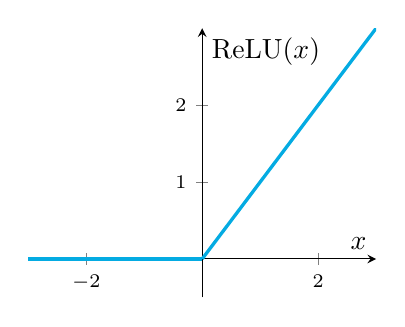
\begin{tikzpicture}
\begin{axis}[width=6cm,height=5cm,axis lines=middle,
	xlabel=$x$,ylabel={$\relu(x)$},
	xmin=-3,xmax=3,ymin=-0.5,ymax=3,
	xtick={-2,0,2},ytick={0,1,2},
	tick label style={font=\scriptsize}]
\addplot[UCMBlue,very thick,domain=-3:0,samples=2]{0};
\addplot[UCMBlue,very thick,domain=0:3,samples=2]{x};
\end{axis}
\end{tikzpicture}
\end{center}
\end{column}
\end{columns}
\end{frame}

\begin{frame}
\frametitle{Sigmoide: la funci\'on de aplastamiento}
\begin{columns}[T]
\begin{column}{6cm}
\formula{\[ \operatorname{sigmoid}(x)=\frac{1}{1+e^{-x}} \]}
\begin{itemize}
	\item Comprime $\R$ al intervalo $(0,1)$: \'util para interpretar salidas como \emph{probabilidades}.
	\item Derivada: $\dfrac{d}{dx}\operatorname{sigmoid}(x)=\operatorname{sigmoid}(x)\big(1-\operatorname{sigmoid}(x)\big)$.
	\pause
	\item \textbf{Problema}: para $|x|$ grande la derivada $\to 0$ $\Rightarrow$ \emph{gradiente se desvanece}.
	\item Hoy se usa poco en capas ocultas; sobrevive en compuertas (LSTM/GRU) y en la salida binaria.
\end{itemize}
\end{column}
\begin{column}{5.5cm}
\begin{center}
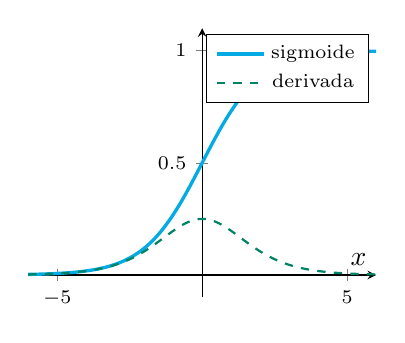
\begin{tikzpicture}
\begin{axis}[width=6cm,height=5cm,axis lines=middle,
	xlabel=$x$,ylabel={$\operatorname{sigmoid}(x)$},
	xmin=-6,xmax=6,ymin=-0.1,ymax=1.1,
	ytick={0,0.5,1},tick label style={font=\scriptsize}]
\addplot[UCMBlue,very thick,domain=-6:6,samples=200]{1/(1+exp(-x))};
\addplot[AccentGreen,thick,dashed,domain=-6:6,samples=200]
	{(1/(1+exp(-x)))*(1-(1/(1+exp(-x))))};
\legend{\scriptsize sigmoide,\scriptsize derivada}
\end{axis}
\end{tikzpicture}
\end{center}
\end{column}
\end{columns}
\end{frame}

\begin{frame}
\frametitle{Tangente hiperb\'olica (tanh)}
\begin{columns}[T]
\begin{column}{6cm}
\formula{\[ \tanh(x)=\frac{1-e^{-2x}}{1+e^{-2x}} \]}
\begin{itemize}
	\item Comprime $\R$ al intervalo $(-1,1)$ y es \textbf{sim\'etrica} respecto al origen.
	\item Derivada: $\dfrac{d}{dx}\tanh(x)=1-\tanh^2(x)$.
	\pause
	\item Al estar centrada en cero suele converger mejor que la sigmoide.
	\item Comparte el problema de saturaci\'on para $|x|$ grande.
\end{itemize}
\end{column}
\begin{column}{5.5cm}
\begin{center}
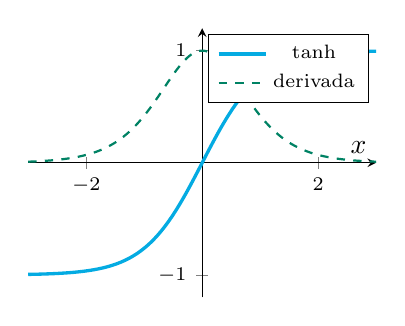
\begin{tikzpicture}
\begin{axis}[width=6cm,height=5cm,axis lines=middle,
	xlabel=$x$,ylabel={$\tanh(x)$},
	xmin=-3,xmax=3,ymin=-1.2,ymax=1.2,
	ytick={-1,0,1},tick label style={font=\scriptsize}]
\addplot[UCMBlue,very thick,domain=-3:3,samples=200]{tanh(x)};
\addplot[AccentGreen,thick,dashed,domain=-3:3,samples=200]{1-tanh(x)^2};
\legend{\scriptsize tanh,\scriptsize derivada}
\end{axis}
\end{tikzpicture}
\end{center}
\end{column}
\end{columns}
\end{frame}

%=====================================================================
\section{Propagaci\'on hacia adelante y hacia atr\'as}
%=====================================================================

\begin{frame}
\frametitle{Propagaci\'on hacia adelante (\emph{forward})}
Calcular y almacenar, en orden, las variables intermedias de la red. Para un ejemplo $\x$ y una capa oculta (sin sesgos, por brevedad):
\begin{align*}
\bm{z}     &= \W^{(1)}\x                    & \text{(pre-activaci\'on)}\\
\h         &= \sigma(\bm{z})                & \text{(activaci\'on oculta)}\\
\bm{o}     &= \W^{(2)}\h                    & \text{(salida)}\\
L          &= \ell(\bm{o}, y)              & \text{(p\'erdida)}\\
s          &= \tfrac{\lambda}{2}\big(\|\W^{(1)}\|_F^2 + \|\W^{(2)}\|_F^2\big) & \text{(regularizaci\'on $L_2$)}\\
J          &= L + s                        & \text{(funci\'on objetivo)}
\end{align*}
\pause
\begin{block}{Grafo computacional}
Representamos el c\'alculo como un grafo dirigido: los \emph{nodos} son variables y operaciones, las \emph{aristas} las dependencias. Es la base de la \emph{diferenciaci\'on autom\'atica}.
\end{block}
\end{frame}

\begin{frame}
\frametitle{Grafo computacional}
\begin{center}
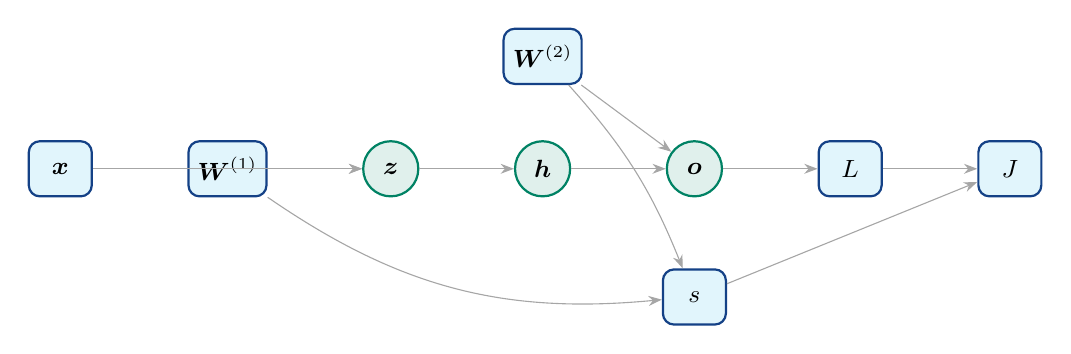
\begin{tikzpicture}[node distance=1.1cm and 1.2cm,
	var/.style={draw=UCMNavy,thick,rounded corners,fill=UCMBlue!12,minimum height=7mm,minimum width=8mm,font=\small},
	op/.style={draw=AccentGreen,thick,circle,fill=AccentGreen!12,minimum size=7mm,font=\small},
	every edge/.style={draw,->,>=Stealth,gray!70}]
\node[var] (x) {$\x$};
\node[var,right=of x] (W1) {$\W^{(1)}$};
\node[op,right=of W1] (z) {$\bm{z}$};
\node[op,right=of z] (h) {$\h$};
\node[var,above=0.7cm of h] (W2) {$\W^{(2)}$};
\node[op,right=of h] (o) {$\bm{o}$};
\node[var,right=of o] (L) {$L$};
\node[var,below=0.9cm of o] (s) {$s$};
\node[var,right=of L] (J) {$J$};
\draw (x) edge (z);
\draw (W1) edge (z);
\draw (z) edge (h);
\draw (h) edge (o);
\draw (W2) edge (o);
\draw (o) edge (L);
\draw (W1) edge[bend right=20] (s);
\draw (W2) edge[bend left=10] (s);
\draw (L) edge (J);
\draw (s) edge (J);
\end{tikzpicture}
\end{center}
\vspace{0.4em}
\footnotesize El paso \emph{forward} recorre el grafo de izquierda a derecha. La \emph{retropropagaci\'on} lo recorre en sentido inverso, acumulando gradientes con la regla de la cadena.
\end{frame}

\begin{frame}
\frametitle{Retropropagaci\'on (\emph{backpropagation})}
M\'etodo para calcular el gradiente de $J$ respecto de los par\'ametros, aplicando la \textbf{regla de la cadena} en orden inverso al \emph{forward}.
\pause
\begin{itemize}
	\item Para una composici\'on $\bm{z}=g(\bm{y})$, $\bm{y}=f(\bm{x})$, la regla de la cadena en forma matricial es:
	\formula{\[
	\frac{\partial \bm{z}}{\partial \bm{x}}
	= \frac{\partial \bm{z}}{\partial \bm{y}}\,\frac{\partial \bm{y}}{\partial \bm{x}}.
	\]}
	\pause
	\item Se parte del objetivo $J$ y se propaga hacia atr\'as:
	\begin{align*}
	\frac{\partial J}{\partial \bm{o}} &= \frac{\partial L}{\partial \bm{o}}, &
	\frac{\partial J}{\partial \W^{(2)}} &= \frac{\partial J}{\partial \bm{o}}\,\h^\top + \lambda\,\W^{(2)},\\
	\frac{\partial J}{\partial \h} &= {\W^{(2)}}^{\!\top}\frac{\partial J}{\partial \bm{o}}, &
	\frac{\partial J}{\partial \bm{z}} &= \frac{\partial J}{\partial \h}\odot \sigma'(\bm{z}).
	\end{align*}
	($\odot$ = producto elemento a elemento).
\end{itemize}
\end{frame}

\begin{frame}
\frametitle{Entrenar la red: \emph{forward} + \emph{backward}}
\begin{algorithmic}[1]
\STATE Inicializar los par\'ametros $\W^{(1)},\W^{(2)},\ldots$ (ver inicializaci\'on).
\FOR{cada \'epoca}
  \FOR{cada \emph{minibatch} $(\X,\bm{y})$}
    \STATE \textbf{Forward}: calcular activaciones y la p\'erdida $J$, almacenando las intermedias.
    \STATE \textbf{Backward}: retropropagar para obtener $\partial J/\partial \W^{(l)}$.
    \STATE \textbf{Actualizar}: $\W^{(l)} \leftarrow \W^{(l)} - \eta\,\partial J/\partial \W^{(l)}$.
  \ENDFOR
\ENDFOR
\end{algorithmic}
\vspace{0.6em}
\begin{itemize}
	\item \emph{Forward} y \emph{backward} se \textbf{alternan} y dependen entre s\'i.
	\pause
	\item Hay que \textbf{retener} en memoria las variables intermedias del \emph{forward} hasta completar el \emph{backward}: por eso entrenar consume mucha m\'as memoria que predecir.
\end{itemize}
\end{frame}

%=====================================================================
\section{Estabilidad num\'erica e inicializaci\'on}
%=====================================================================

\begin{frame}
\frametitle{Gradientes que se desvanecen o explotan}
El gradiente en una red de $L$ capas es un \textbf{producto} de $L$ matrices jacobianas:
\formula{\[
\frac{\partial J}{\partial \W^{(l)}} \;\propto\;
\prod_{k=l}^{L-1}\frac{\partial \h^{(k+1)}}{\partial \h^{(k)}}.
\]}
\begin{itemize}
	\item \textbf{Explosi\'on}: si los factores son $>1$, el producto crece exponencialmente $\Rightarrow$ par\'ametros divergen.
	\pause
	\item \textbf{Desvanecimiento}: si los factores son $<1$, el producto $\to 0$ $\Rightarrow$ las capas iniciales dejan de aprender.
	\pause
	\item La sigmoide es un culpable cl\'asico: su derivada m\'axima es $0.25$ y se anula en las colas (ver siguiente l\'amina).
\end{itemize}
\end{frame}

\begin{frame}
\frametitle{El gradiente de la sigmoide se anula en las colas}
\begin{center}
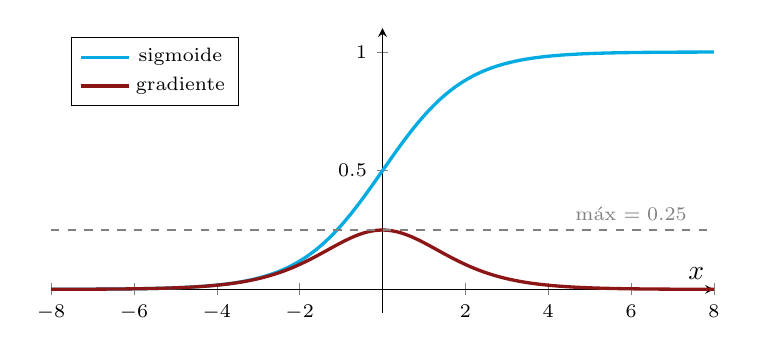
\begin{tikzpicture}
\begin{axis}[width=10cm,height=5.2cm,axis lines=middle,
	xlabel=$x$,ylabel={},xmin=-8,xmax=8,ymin=-0.1,ymax=1.1,
	legend pos=north west,tick label style={font=\scriptsize}]
\addplot[UCMBlue,very thick,domain=-8:8,samples=200]{1/(1+exp(-x))};
\addplot[StanfordRed,very thick,domain=-8:8,samples=200]
	{(1/(1+exp(-x)))*(1-(1/(1+exp(-x))))};
\legend{\scriptsize sigmoide,\scriptsize gradiente}
\draw[gray,dashed] (axis cs:-8,0.25)--(axis cs:8,0.25);
\node[gray,font=\scriptsize] at (axis cs:6,0.32){m\'ax $=0.25$};
\end{axis}
\end{tikzpicture}
\end{center}
\vspace{0.2em}
\footnotesize Cuando la entrada es muy positiva o muy negativa, el gradiente es pr\'acticamente nulo: la retropropagaci\'on puede ``estancarse''. ReLU evita esto en su rama positiva.
\end{frame}

\begin{frame}
\frametitle{Romper la simetr\'ia e inicializar bien}
\begin{block}{Simetr\'ia}
Si todos los pesos se inicializan \textbf{iguales} (p.~ej. a cero), todas las unidades de una capa calculan lo mismo y reciben el mismo gradiente: nunca se diferencian. Hay que inicializar de forma \textbf{aleatoria}.
\end{block}
\pause
\begin{itemize}
	\item \textbf{Inicializaci\'on de Xavier (Glorot)}: elige la varianza de los pesos para mantener estable la magnitud de activaciones y gradientes a trav\'es de las capas.
	\formula{\[
	\Var(w) = \frac{2}{n_{\text{ent}}+n_{\text{sal}}}
	\quad\Longleftrightarrow\quad
	w \sim U\!\left(-\sqrt{\tfrac{6}{n_{\text{ent}}+n_{\text{sal}}}},\; \sqrt{\tfrac{6}{n_{\text{ent}}+n_{\text{sal}}}}\right).
	\]}
	donde $n_{\text{ent}}$ y $n_{\text{sal}}$ son el n\'umero de entradas y salidas de la capa.
	\pause
	\item Para ReLU se suele usar la variante \emph{He}, con varianza $2/n_{\text{ent}}$.
\end{itemize}
\end{frame}

%=====================================================================
\section{Generalizaci\'on y regularizaci\'on}
%=====================================================================

\begin{frame}
\frametitle{Sobreajuste en redes profundas}
\begin{itemize}
	\item Las redes profundas tienen \textbf{enorme capacidad}: pueden memorizar incluso etiquetas aleatorias.
	\pause
	\item Por ello la \emph{brecha de generalizaci\'on} (diferencia entre error de entrenamiento y de prueba) es una preocupaci\'on central.
	\pause
	\item Herramientas para mejorar la generalizaci\'on:
	\begin{itemize}
		\item \textbf{Detenci\'on temprana} (\emph{early stopping}).
		\item \textbf{Decaimiento de pesos} (regularizaci\'on $L_2$).
		\item \textbf{Dropout}.
		\item M\'as datos y \emph{data augmentation}.
	\end{itemize}
\end{itemize}
\end{frame}

\begin{frame}
\frametitle{Detenci\'on temprana y decaimiento de pesos}
\begin{columns}[T]
\begin{column}{6cm}
\textbf{Detenci\'on temprana}
\begin{itemize}
	\item Monitorear el error de validaci\'on durante el entrenamiento.
	\item Detener cuando el error de validaci\'on deja de mejorar, aunque el de entrenamiento siga bajando.
	\item Limita de hecho el n\'umero de \'epocas: una forma impl\'icita de regularizaci\'on.
\end{itemize}
\end{column}
\begin{column}{6cm}
\textbf{Decaimiento de pesos ($L_2$)}
\begin{itemize}
	\item A\~nade una penalizaci\'on a la norma de los pesos:
	\formula{\[ J = L + \frac{\lambda}{2}\sum_l \|\W^{(l)}\|_F^2. \]}
	\item Favorece pesos peque\~nos $\Rightarrow$ funciones m\'as suaves.
	\item $\lambda$ controla la fuerza de la regularizaci\'on.
\end{itemize}
\end{column}
\end{columns}
\end{frame}

%=====================================================================
\section{Dropout}
%=====================================================================

\begin{frame}
\frametitle{Dropout: la idea}
\begin{itemize}
	\item Durante el entrenamiento, \textbf{desactivar} al azar una fracci\'on $p$ de las neuronas en cada paso.
	\pause
	\item Impide que las unidades \emph{co-adapten}: ninguna puede depender de la presencia de otra concreta $\Rightarrow$ representaciones m\'as robustas.
	\pause
	\item Equivale aproximadamente a entrenar y promediar un \emph{ensamble} enorme de subredes que comparten pesos.
\end{itemize}
\pause
\begin{block}{Dropout invertido (\emph{en la pr\'actica})}
Cada activaci\'on $h$ se reemplaza por
\[
h' =
\begin{cases}
0 & \text{con probabilidad } p,\\[2pt]
\dfrac{h}{1-p} & \text{en caso contrario.}
\end{cases}
\]
As\'i $\E[h']=h$: la salida esperada no cambia y no hay que reescalar al predecir.
\end{block}
\end{frame}

\begin{frame}
\frametitle{Dropout: red completa vs. red con unidades apagadas}
\begin{columns}[c]
\begin{column}{6cm}
\begin{center}
\textbf{Sin dropout}\\[2mm]
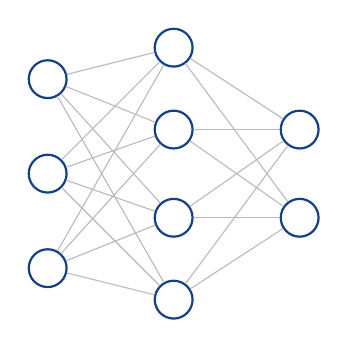
\begin{tikzpicture}[scale=0.8,transform shape,
	neuron/.style={circle,draw=UCMNavy,thick,minimum size=6mm},
	off/.style={circle,draw=gray!50,dashed,fill=gray!10,minimum size=6mm}]
\foreach \i/\y in {1/1.5,2/0,3/-1.5}\node[neuron] (I\i) at (0,\y){};
\foreach \i/\y in {1/2,2/0.7,3/-0.7,4/-2}\node[neuron] (H\i) at (2,\y){};
\foreach \i/\y in {1/0.7,2/-0.7}\node[neuron] (O\i) at (4,\y){};
\foreach \a in {1,2,3}\foreach \b in {1,2,3,4}\draw[gray!55] (I\a)--(H\b);
\foreach \a in {1,2,3,4}\foreach \b in {1,2}\draw[gray!55] (H\a)--(O\b);
\end{tikzpicture}
\end{center}
\end{column}
\begin{column}{6cm}
\begin{center}
\textbf{Con dropout}\\[2mm]
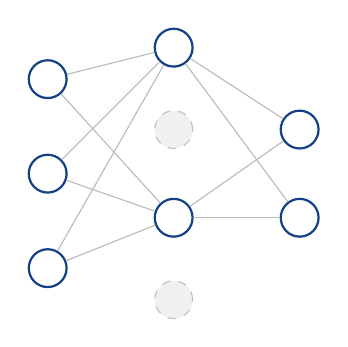
\begin{tikzpicture}[scale=0.8,transform shape,
	neuron/.style={circle,draw=UCMNavy,thick,minimum size=6mm},
	off/.style={circle,draw=gray!50,dashed,fill=gray!12,minimum size=6mm}]
\foreach \i/\y in {1/1.5,2/0,3/-1.5}\node[neuron] (I\i) at (0,\y){};
\node[neuron] (H1) at (2,2){};
\node[off]    (H2) at (2,0.7){};
\node[neuron] (H3) at (2,-0.7){};
\node[off]    (H4) at (2,-2){};
\foreach \i/\y in {1/0.7,2/-0.7}\node[neuron] (O\i) at (4,\y){};
\foreach \a in {1,2,3}\foreach \b in {1,3}\draw[gray!55] (I\a)--(H\b);
\foreach \a in {1,3}\foreach \b in {1,2}\draw[gray!55] (H\a)--(O\b);
\end{tikzpicture}
\end{center}
\end{column}
\end{columns}
\vspace{0.6em}
\footnotesize En cada paso de entrenamiento se apaga un subconjunto distinto de neuronas (en gris). Al \textbf{predecir}, dropout se desactiva y se usa la red completa.
\end{frame}

\begin{frame}
\frametitle{Resumen}
\begin{center}
\begin{tabular}{ll}
\toprule
\textbf{Concepto} & \textbf{Idea clave}\\
\midrule
MLP             & Capas totalmente conectadas + no linealidad\\
Activaci\'on    & ReLU por defecto; sigmoide/tanh saturan\\
No linealidad   & Sin ella, la red colapsa a un modelo lineal\\
Backprop        & Regla de la cadena en sentido inverso\\
Estabilidad     & Gradientes que se desvanecen / explotan\\
Inicializaci\'on& Romper simetr\'ia; Xavier/He\\
Regularizaci\'on& \emph{Early stopping}, $L_2$, dropout\\
\bottomrule
\end{tabular}
\end{center}
\vspace{0.8em}
\begin{itemize}
	\item Un MLP es la red profunda m\'as simple, pero ya contiene \textbf{todas} las ideas centrales: capas, no linealidad, retropropagaci\'on y regularizaci\'on.
	\item Estas bases se reutilizan en CNN, RNN y \emph{transformers}.
\end{itemize}
\end{frame}

\begin{frame}
\frametitle{Para profundizar}
\begin{itemize}
	\item Zhang, Lipton, Li \& Smola, \emph{Dive into Deep Learning}, cap.~5 (Multilayer Perceptrons)\\ \url{https://d2l.ai/chapter_multilayer-perceptrons/index.html}
	\item Goodfellow, Bengio \& Courville, \emph{Deep Learning} (cap.~6, \emph{Deep Feedforward Networks})\\ \url{https://www.deeplearningbook.org/}
	\item Glorot \& Bengio (2010), \emph{Understanding the difficulty of training deep feedforward neural networks}.
	\item Srivastava et al.\ (2014), \emph{Dropout: A Simple Way to Prevent Neural Networks from Overfitting}.
	\item Documentaci\'on de PyTorch: \emph{torch.nn}\\ \url{https://pytorch.org/docs/stable/nn.html}
\end{itemize}
\end{frame}

\end{document}
